%!TeX root=../acctop.tex
\addchap[Stave V: The End of It]{{\moderatelyhuge Stave Five}\\The End of It}
\begin{minipage}[c]{\textwidth}

\includegraphics[width=\textwidth]{snapdragonimproved}
\captionof{figure}[Headpiece to Stave V]{}
\end{minipage}

\lettrine[lines=4]{Y}{es!} and the bedpost was his own. The bed was his own, the room was his own. Best and happiest of all, the Time before him was his own, to make amends in!

\makeatletter
\@ifclasswith{scrbook}{a5paper}
{%
»I will live in the Past, the Present, and the Future!« Scrooge repeated as he scrambled out of bed. »The Spirits of all Three shall strive within me. O Jacob Marley! Heaven and the Christmas Time be praised for this! I say it on my knees, old Jacob; on my knees!«

}{%
\zz
»I will live in the Past, the Present, and the Future!« Scrooge repeated as he scrambled out of bed. »The Spirits of all Three shall strive within me. O Jacob Marley! Heaven and the Christmas Time be praised for this! I say it on my knees, old Jacob; on my knees!«
}
\makeatother


»I will live in the Past, the Present, and the Future!« Scrooge repeated as he scrambled out of bed. »The Spirits of all Three shall strive within me. O Jacob Marley! Heaven and the Christmas Time be praised for this! I say it on my knees, old Jacob; on my knees!«

He was so fluttered and so glowing with his good intentions, that his broken voice would scarcely answer to his call. He had been sobbing violently in his conflict with the Spirit, and his face was wet with tears.

»They are not torn down,« cried Scrooge, folding one of his bed-curtains in his arms, »They are not torn down, rings and all. They are here—I am here—the shadows of the things that would have been may be dispelled. They will be. I know they will!«

His hands were busy with his garments all this time: turning them inside out, putting them on upside down, tearing them, mislaying them, making them parties to every kind of extravagance.

»I don't know what to do!« cried Scrooge, laughing and crying in the same breath, and making a perfect Laoco\"on of himself with his stockings. »I am as light as a feather, I am as happy as an angel, I am as merry as a schoolboy, I am as giddy as a drunken man. A merry Christmas to everybody! A happy New Year to all the world! Hallo here! Whoop! Hallo!«

He had frisked into the sitting-room, and was now standing there, perfectly winded.

»There's the saucepan that the gruel was in!« cried Scrooge, starting off again, and going round the fireplace. »There's the door by which the Ghost of Jacob Marley entered! There's the corner where the Ghost of Christmas Present sat! There's the window where I saw the wandering Spirits! It's all right, it's all true, it all happened. Ha, ha, ha!«

Really, for a man who had been out of practice for so many years, it was a splendid laugh, a most illustrious laugh. The father of a long, long line of brilliant laughs!

»I don't know what day of the month it is,« said Scrooge. »I don't know how long I have been among the Spirits. I don't know anything. I'm quite a baby. Never mind. I don't care. I'd rather be a baby. Hallo! Whoop! Hallo here!«

He was checked in his transports by the churches ringing out the lustiest peals he had ever heard. Clash, clash, hammer; ding, dong, bell! Bell, dong, ding; hammer, clash, clash! Oh, glorious, glorious!

Running to the window, he opened it, and put out his head. No fog, no mist; clear, bright, jovial, stirring, cold; cold, piping for the blood to dance to; golden sunlight; heavenly sky; sweet fresh air; merry bells. Oh, glorious! Glorious!

»What's to-day?« cried Scrooge, calling downward to a boy in Sunday clothes, who perhaps had loitered in to look about him.

»Eh?« returned the boy with all his might of wonder.

»What's to-day, my fine fellow?« said Scrooge.

»To-day!« replied the boy. »Why, \textsc{Christmas Day.}«

»It's Christmas Day!« said Scrooge to himself. »I haven't missed it. The Spirits have done it all in one night. They can do anything they like. Of course they can. Of course they can. Hallo, my fine fellow!«

»Hallo!« returned the boy.

»Do you know the poulterer's in the next street but one, at the corner?« Scrooge inquired.

»I should hope I did,« replied the lad.

»An intelligent boy!« said Scrooge. »A remarkable boy! Do you know whether they've sold the prize turkey that was hanging up there?—Not the little prize turkey: the big one?«

»What! the one as big as me?« returned the boy.

»What a delightful boy!« said Scrooge. »It's a pleasure to talk to him. Yes, my buck!«

»It's hanging there now,« replied the boy.

»Is it?« said Scrooge. »Go and buy it.«

\begin{center}
\begin{minipage}[c]{\textwidth}
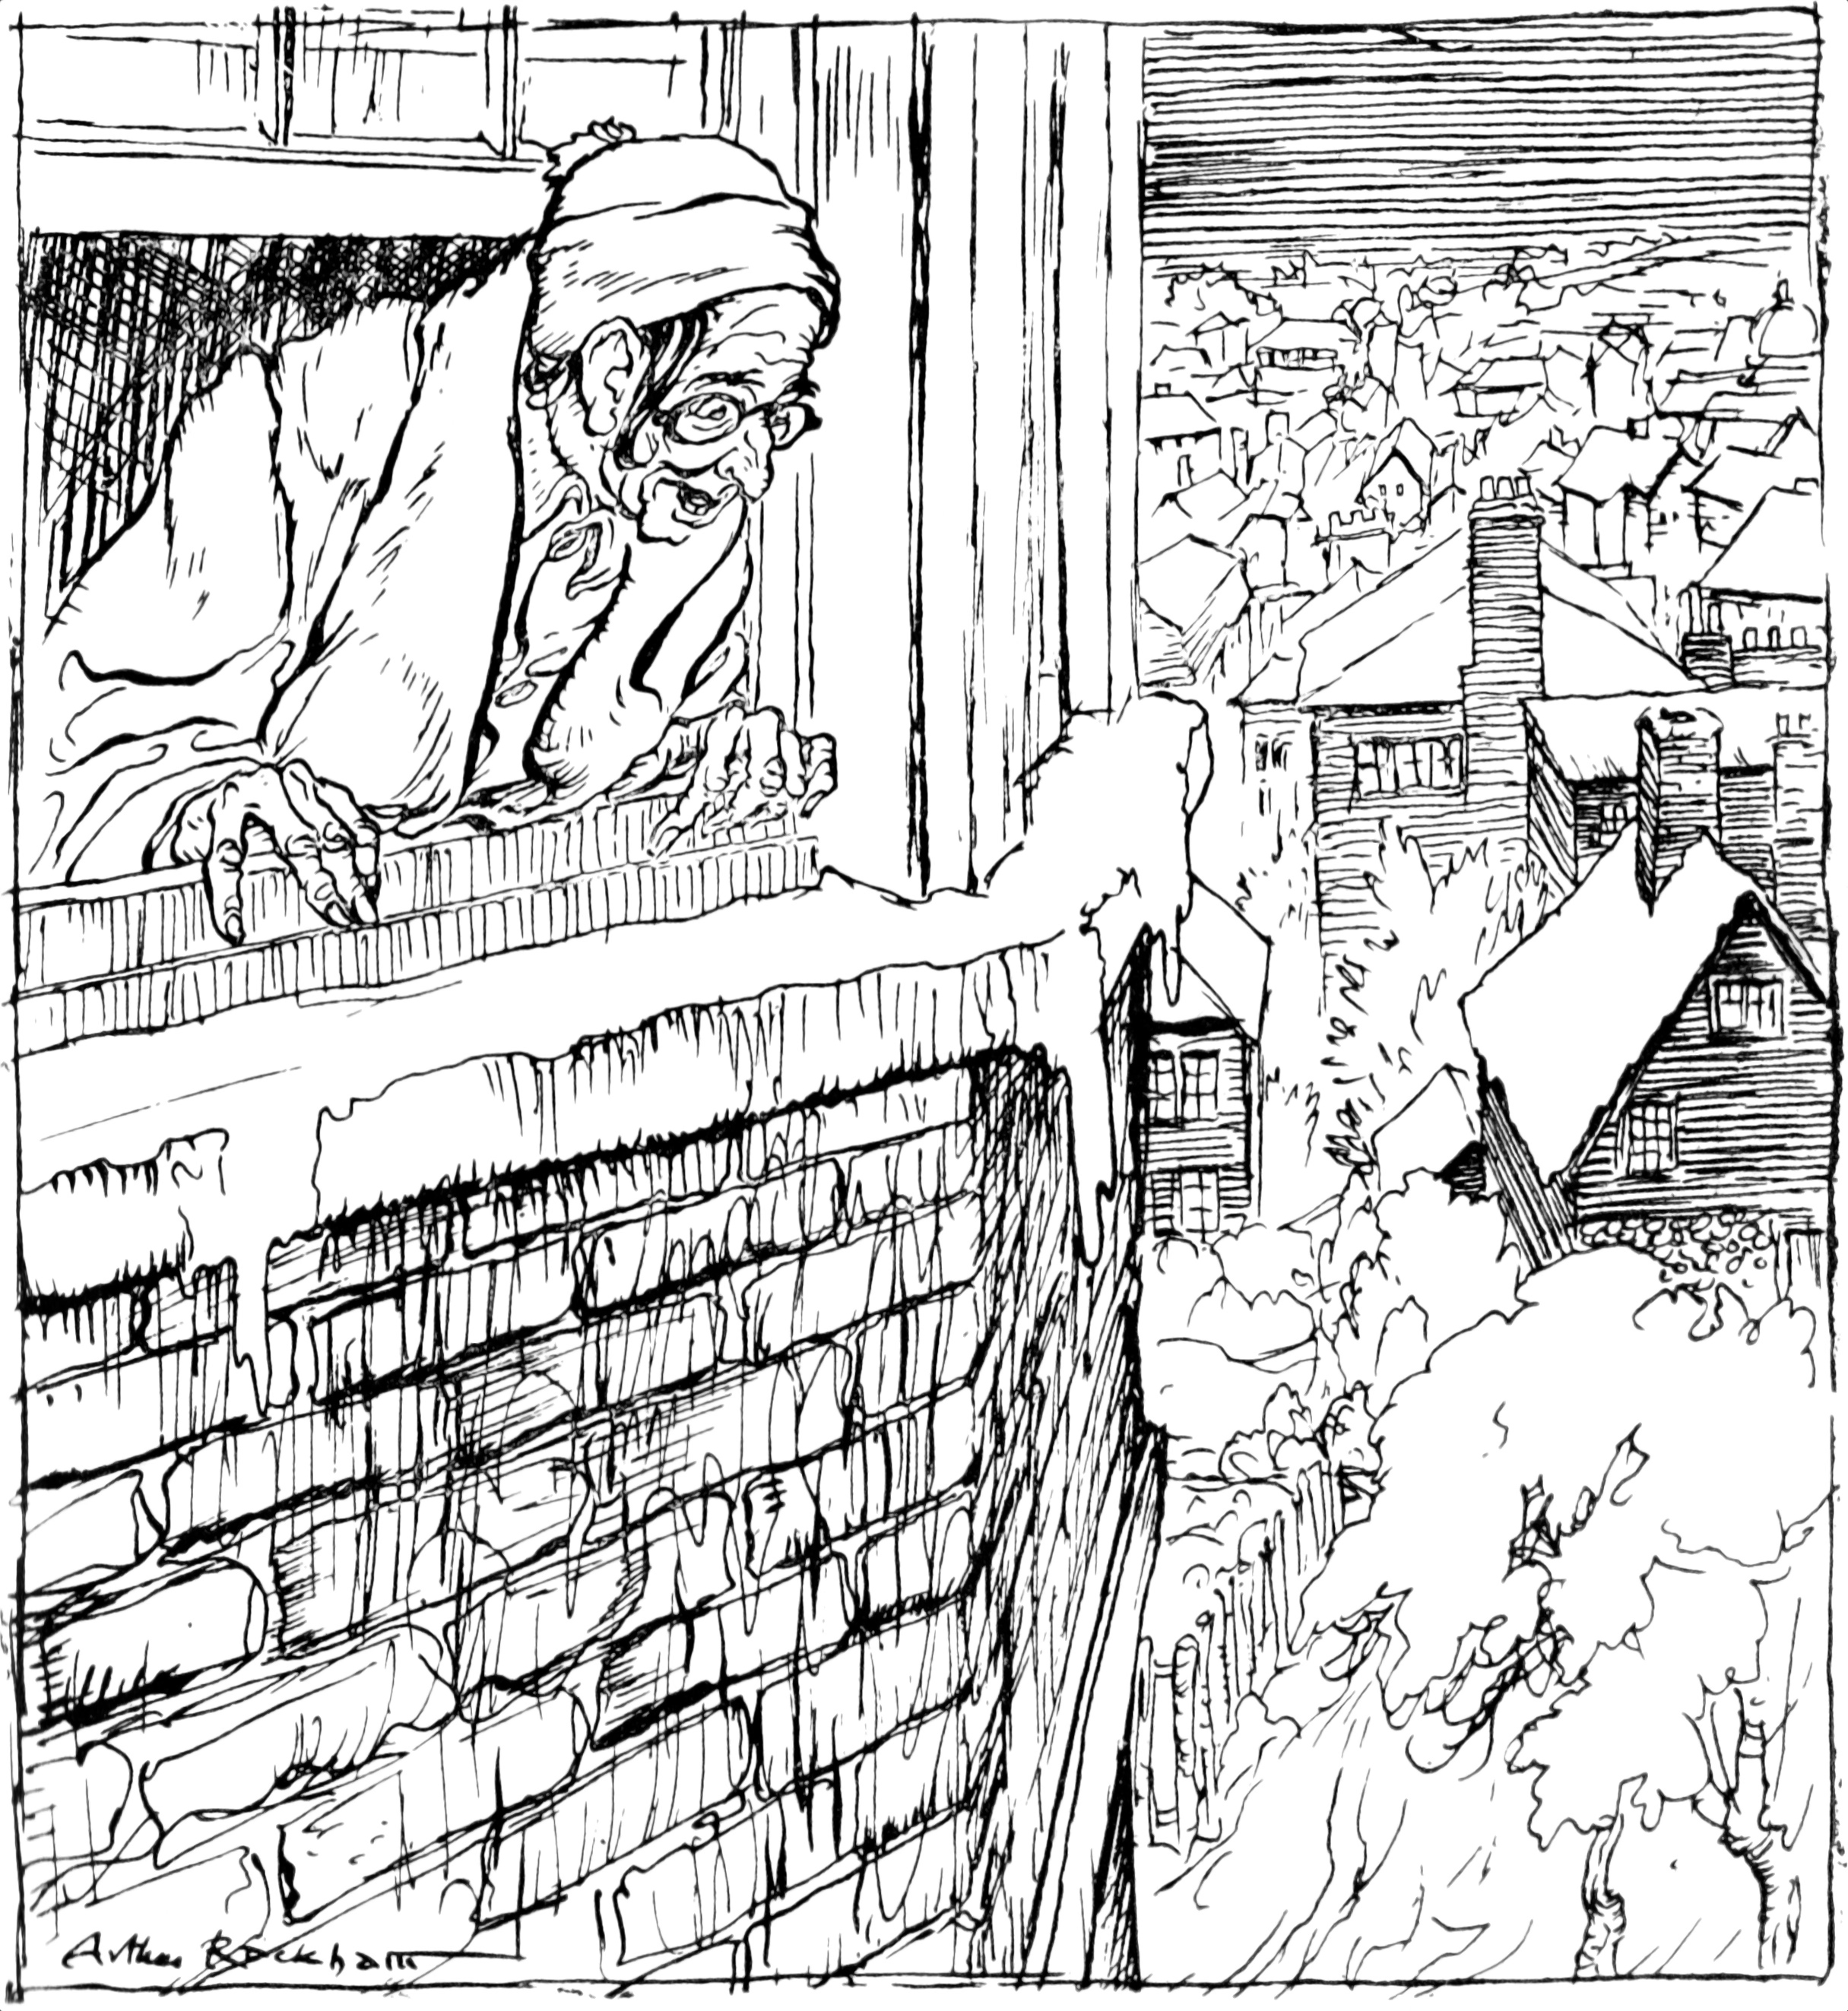
\includegraphics[width=\textwidth]{whatday}
\captionof{figure}{»What's to-day?« cried Scrooge.}
\end{minipage}
\end{center}

\enquote{Walk-\textsc{er}!} exclaimed the boy.

»No, no,« said Scrooge. »I am in earnest. Go and buy it, and tell `em to bring it here, that I may give them the directions where to take it. Come back with the man, and I'll give you a shilling. Come back with him in less than five minutes, and I'll give you half-a-crown!«

The boy was off like a shot. He must have had a steady hand at a trigger who could have got a shot off half as fast.

»I'll send it to Bob Cratchit's,« whispered Scrooge, rubbing his hands, and splitting with a laugh. »He shan't know who sends it. It's twice the size of Tiny Tim. Joe Miller never made such a joke as sending it to Bob's will be!«

The hand in which he wrote the address was not a steady one; but write it he did, somehow, and went downstairs to open the street-door, ready for the coming of the poulterer's man. As he stood there, waiting his arrival, the knocker caught his eye.

»I shall love it as long as I live!« cried Scrooge, patting it with his hand. »I scarcely ever looked at it before. What an honest expression it has in its face! It's a wonderful knocker!—Here's the turkey. Hallo! Whoop! How are you! Merry Christmas!«

It \textit{was} a turkey! He never could have stood upon his legs, that bird. He would have snapped `em short off in a minute, like sticks of sealing-wax.

»Why, it's impossible to carry that to Camden Town,« said Scrooge. »You must have a cab.«

The chuckle with which he said this, and the chuckle with which he paid for the turkey, and the chuckle with which he paid for the cab, and the chuckle with which he recompensed the boy, were only to be exceeded by the chuckle with which he sat down breathless in his chair again, and chuckled till he cried.

Shaving was not an easy task, for his hand continued to shake very much; and shaving requires attention, even when you don't dance while you are at it. But if he had cut the end of his nose off, he would have put a piece of sticking-plaster over it, and been quite satisfied.

He dressed himself »all in his best,« and at last got out into the streets. The people were by this time pouring forth, as he had seen them with the Ghost of Christmas Present; and, walking with his hands behind him, Scrooge regarded every one with a delighted smile. He looked so irresistibly pleasant, in a word, that three or four good-humoured fellows said, »Good-morning, sir! A merry Christmas to you!« And Scrooge said often afterwards that, of all the blithe sounds he had ever heard, those were the blithest in his ears.

He had not gone far when, coming on towards him, he beheld the portly gentleman who had walked into his counting-house the day before, and said, »Scrooge and Marley's, I believe?« It sent a pang across his heart to think how this old gentleman would look upon him when they met; but he knew what path lay straight before him, and he took it.

»My dear sir,« said Scrooge, quickening his pace, and taking the old gentleman by both his hands, »how do you do? I hope you succeeded yesterday. It was very kind of you. A merry Christmas to you, sir!«

\begin{figure}[p]
\begin{minipage}[c]{\textwidth}
\includegraphics[width=\textwidth]{freddinnerimproved}
\caption[\textbf{»Will you let me in, Fred?«}]{»It's I, your uncle Scrooge. I have come to dinner. Will you let me in, Fred?«}
\end{minipage}
\end{figure}

»Mr Scrooge?«

»Yes,« said Scrooge. »That is my name, and I fear it may not be pleasant to you. Allow me to ask your pardon. And will you have the goodness\longdash« Here Scrooge whispered in his ear.

»Lord bless me!« cried the gentleman, as if his breath were taken away. »My dear Mr Scrooge, are you serious?«

»If you please,« said Scrooge. »Not a farthing less. A great many back-payments are included in it, I assure you. Will you do me that favour?«

»My dear sir,« said the other, shaking hands with him, »I don't know what to say to such munifi\longdash«

»Don't say anything, please,« retorted Scrooge. »Come and see me. Will you come and see me?«

»I will!« cried the old gentleman. And it was clear he meant to do it.

»Thankee,« said Scrooge. »I am much obliged to you. I thank you fifty times. Bless you!«

He went to church, and walked about the streets, and watched the people hurrying to and fro, and patted the children on the head, and questioned beggars, and looked down into the kitchens of houses, and up to the windows; and found that everything could yield him pleasure. He had never dreamed that any walk—that anything—could give him so much happiness. In the afternoon he turned his steps towards his nephew's house.

He passed the door a dozen times before he had the courage to go up and knock. But he made a dash and did it.

»Is your master at home, my dear?« said Scrooge to the girl. »Nice girl! Very.«

»Yes, sir.«

»Where is he, my love?« said Scrooge.

»He's in the dining-room, sir, along with mistress. I'll show you upstairs, if you please.«

»Thankee. He knows me,« said Scrooge, with his hand already on the dining-room lock. »I'll go in here, my dear.«

He turned it gently, and sidled his face in round the door. They were looking at the table (which was spread out in great array); for these young housekeepers are always nervous on such points, and like to see that everything is right.

»Fred!« said Scrooge.

Dear heart alive, how his niece by marriage started! Scrooge had forgotten, for the moment, about her sitting in the corner with the footstool, or he wouldn't have done it on any account.

»Why, bless my soul!« cried Fred, »who's that?«

»It's I. Your uncle Scrooge. I have come to dinner. Will you let me in, Fred?«

Let him in! It is a mercy he didn't shake his arm off. He was at home in five minutes. Nothing could be heartier. His niece looked just the same. So did Topper when \textit{he} came. So did the plump sister when \textit{she} came. So did every one when \textit{they} came. Wonderful party, wonderful games, wonderful unanimity, won-der-ful happiness!

But he was early at the office next morning. Oh, he was early there! If he could only be there first, and catch Bob Cratchit coming late! That was the thing he had set his heart upon.

\begin{figure}[p]
\begin{minipage}[c]{\textwidth}
\includegraphics[width=\textwidth]{boblate2}
\caption[\textbf{»I am not going to stand this any longer.«}]{»Now, I'll tell you what, my friend,« said Scrooge. »I am not going to stand this sort of thing any longer.«}
\end{minipage}
\end{figure}

And he did it; yes, he did! The clock struck nine. No Bob. A quarter past. No Bob. He was full eighteen minutes and a half behind his time. Scrooge sat with his door wide open, that he might see him come into the tank.

His hat was off before he opened the door; his comforter too. He was on his stool in a jiffy, driving away with his pen, as if he were trying to overtake nine o'clock.

»Hallo!« growled Scrooge in his accustomed voice as near as he could feign it. »What do you mean by coming here at this time of day?«

»I am very sorry, sir,« said Bob. »I \textit{am} behind my time.«

»You are!« repeated Scrooge. »Yes, I think you are. Step this way, sir, if you please.«

»It's only once a year, sir,« pleaded Bob, appearing from the tank. »It shall not be repeated. I was making rather merry yesterday, sir.«

»Now, I'll tell you what, my friend,« said Scrooge. »I am not going to stand this sort of thing any longer. And therefore,« he continued, leaping from his stool, and giving Bob such a dig in the waistcoat that he staggered back into the tank again— »and therefore I am about to raise your salary!«

Bob trembled, and got a little nearer to the ruler. He had a momentary idea of knocking Scrooge down with it, holding him, and calling to the people in the court for help and a strait-waistcoat.

»A merry Christmas, Bob!« said Scrooge, with an earnestness that could not be mistaken, as he clapped him on the back. »A merrier Christmas, Bob, my good fellow, than I have given you for many a year! I'll raise your salary, and endeavour to assist your struggling family, and we will discuss your affairs this very afternoon, over a Christmas bowl of smoking bishop, Bob! Make up the fires and buy another coal-scuttle before you dot another i, Bob Cratchit!«

Scrooge was better than his word. He did it all, and infinitely more; and to Tiny Tim, who did \textsc{not} die, he was a second father. He became as good a friend, as good a master, and as good a man as the good old City knew, or any other good old city, town, or borough in the good old world. Some people laughed to see the alteration in him, but he let them laugh, and little heeded them; for he was wise enough to know that nothing ever happened on this globe, for good, at which some people did not have their fill of laughter in the outset; and knowing that such as these would be blind anyway, he thought it quite as well that they should wrinkle up their eyes in grins as have the malady in less attractive forms. His own heart laughed, and that was quite enough for him.

He had no further intercourse with Spirits, but lived upon the Total-Abstinence Principle ever afterwards; and it was always said of him that he knew how to keep Christmas well, if any man alive possessed the knowledge. May that be truly said of us, and all of us! And so, as Tiny Tim observed, God bless Us, Every One!


\makeatletter
\@ifclasswith{scrbook}{a5paper}
{%
	\begin{center}
		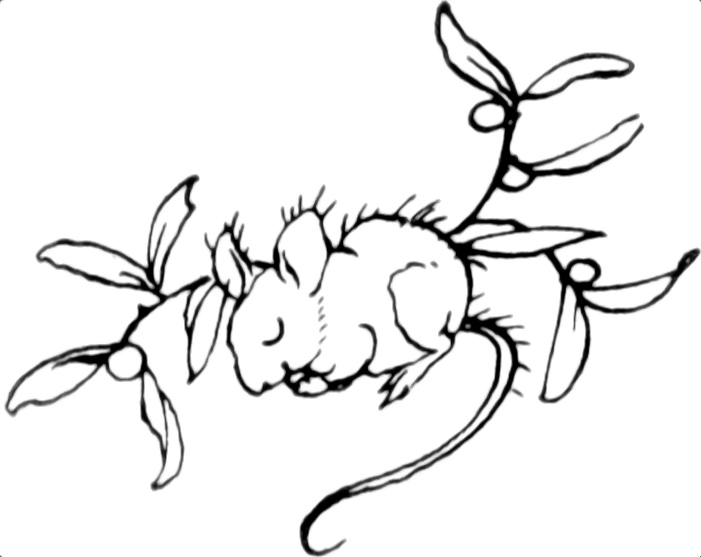
\includegraphics[width=.7\textwidth]{mousie}
		\captionof{figure}[Tailpiece to Stave V]{}
	\end{center}
	\enlargethispage {\baselineskip} 
	\clearpage
}{%
	\begin{center}
		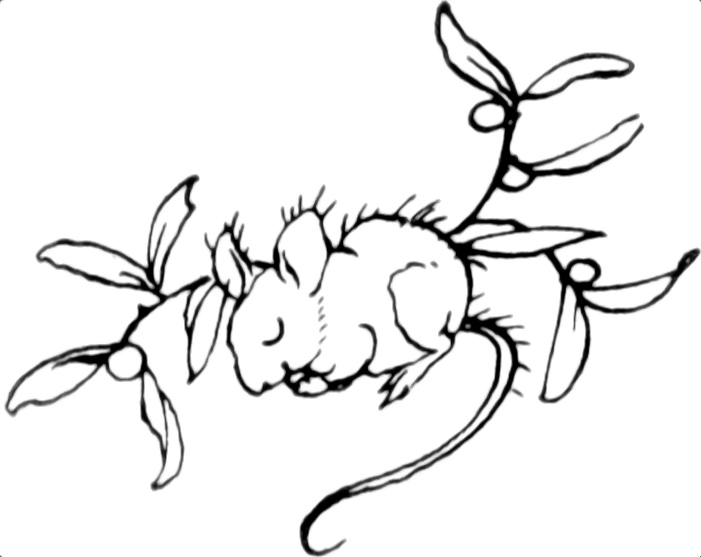
\includegraphics[width=.6\textwidth]{mousie}
		\captionof{figure}[Tailpiece to Stave V]{}
	\end{center}
	\enlargethispage {\baselineskip} 
	\clearpage
}
\makeatother


